\documentclass[a4paper,  11pt]{ctexart}
\usepackage{srcltx,graphicx}
\usepackage{amsmath, amssymb, amsthm}
\usepackage{color}
\usepackage{lscape}
\usepackage{multirow}
\usepackage{psfrag}
\usepackage{diagbox}
\usepackage[hang]{subfigure}
\usepackage{float}
\usepackage[colorlinks,linkcolor=black,anchorcolor=blue,citecolor=green]{hyperref}

\newtheorem{theorem}{Theorem}
\newtheorem{lemma}{Lemma}
\newtheorem{definition}{Definition}
\newtheorem{comment}{Comment}
\newtheorem{conjecture}{Conjecture}

\newcommand\bbR{\mathbb{R}}
\newcommand\bbN{\mathbb{N}}
\newcommand\bbC{\mathbb{C}}
\newcommand\bx{\boldsymbol{x}}
\newcommand\dd{\,\mathrm{d}}

\newcommand\diag{\mathrm{diag}}
\newcommand\tr{\mthrm{tr}}

\setlength{\oddsidemargin}{0cm}
\setlength{\evensidemargin}{0cm}
\setlength{\textwidth}{150mm}
\setlength{\textheight}{230mm}

\newcommand\note[2]{{{\bf #1}\color{red} [ {\it #2} ]}}
%\newcommand\note[2]{{ #1 }} % using this line in the formal version

\newcommand\pd[2]{\dfrac{\partial {#1}}{\partial {#2}}}
\newcommand\od[2]{\dfrac{\dd {#1}}{\dd {#2}}}
\newcommand{\bm}[1]{\mbox{\boldmath{$#1$}}}

\begin{document}
\title{图像处理中的数学方法-homework4}
\author{郑灵超}
\maketitle
%\tableofcontents
%\newpage

\section{算法介绍}
\subsection{TV}
\[  
   \min \lambda \Vert\nabla u\Vert_1 + \frac 12 \Vert
   Au - f \Vert_2^2
\]
我们采用的算法为ADMM算法,其迭代格式如下:
\begin{enumerate}
    \item $u_{k+1}=(A^TA+\mu W^TW)^{-1}(A^Tf+\mu W^T(d_k-b_k)),$
    \item $d_{k+1}=\mathcal{T}_{\bm\lambda/u}(Wu_{k+1}+b_k),$
    \item $b_{k+1}=b_k+\delta(Wu_{k+1}-d_{k+1}).$
\end{enumerate}
迭代的终止条件为
\[
\frac{\Vert Wu_{k+1}-d_{k+1}\Vert_2 }{\Vert f\Vert_2}<tol.
\]
\subsubsection*{算法分析}

算子$A$对应于一个矩阵$A$与$f$的卷积,算子$W^TW$对应于矩阵$L$与$f$的卷
积,
记$\hat{A},\hat{L},\hat{f}$分别为它们的Fourier变换后的矩阵,则迭代格式第一步等
价于

\[
    (\hat{A}*\hat{A}+\mu\hat{L})*\hat{u}_{k+1}=\hat{A}*\hat{f}+\mu
    (W^T(d_k-b_k))^{\hat{} }.
\]
而为了求解迭代过程中的第一个方程,我们采用FFT算法,步骤如下:
其中这里的$*$表示矩阵逐分量相乘。\par
因此我们可以通过如下步骤求解该方程:
\begin{enumerate}
    \item 计算算子$A^TA$和$W^TW$的Fourier变换的矩阵$\hat{A}$与
        $\hat{\Delta}$,以及$\hat{f}$和$W^T(d-b)$的Fourier变换
        $\hat{v}$.
    \item 计算$
        (\hat{A}*\hat{f}+\mu\hat{v})/(\hat{A}*\hat{A}+\mu\hat{L})$,
        这里的$*,/$均表示逐项操作。
    \item 做Fourier逆变换得到$u$.
\end{enumerate}

\subsection{Analysis Based Approach}
\[  
   \min \Vert \lambda \cdot Wu\Vert_1 + \frac 12 \Vert
   Au - f \Vert_2^2
\]
我们采用的算法为ADMM算法,其迭代格式如下:
\begin{enumerate}
    \item $u_{k+1}=(A^TA+\mu)^{-1}(A^Tf+\mu W^T(d_k-b_k)),$
    \item $d_{k+1}=\mathcal{T}_{\bm\lambda/u}(Wu_{k+1}+b_k),$
    \item $b_{k+1}=b_k+\delta(Wu_{k+1}-d_{k+1}).$
\end{enumerate}
迭代的终止条件为
\[
\frac{\Vert Wu_{k+1}-d_{k+1}\Vert_2 }{\Vert f\Vert_2}<tol.
\]
具体算法的实现与TV类似,采用FFT求解方程。
\subsection{Balanced Approach}
\[ 
  \min_{\alpha\in\mathbb{R}^m} \Vert
  \bm\lambda\cdot \alpha\Vert_1 + \frac 12
  \Vert AW^T\alpha-f\Vert_2^2+\frac{\kappa}{2}
  \Vert(I-WW^T)\alpha\Vert_2^2
\]
我们采用的算法为PFBS算法,其迭代格式如下:
\begin{enumerate}
    \item $g_k=\alpha_k-\nabla F_2(\alpha_k)/L$,其中
       $\nabla F_2(\alpha) = WA^T(AW^T\alpha-f)
       +\kappa(I-WW^T)\alpha$.
\end{enumerate}
\section{数值实验}

我们使用的图像为lenna图片,并对其加了模糊和噪声作为待处理图片,加入的
模糊和噪声分别为
\[    
      \sigma_1 = 1.5, \sigma_2 = |u|/10
\]
即
\[  
  f = A\tilde{u} + \sigma_2\text{randn},
\]
其中$A$的卷积核为
\[   
   k = \text{fspecial}("Gaussian",[15,15],sigma_1).
\]
初始图片和待处理图片分别为
\begin{figure}[H]
  \subfigure[原图]{
    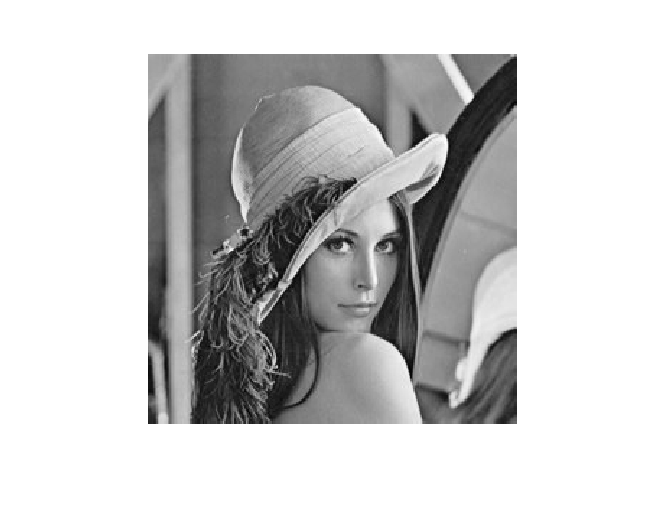
\includegraphics[width=0.45\textwidth]{../program/Lenna.eps}
  }
  \subfigure[待处理图片]{
    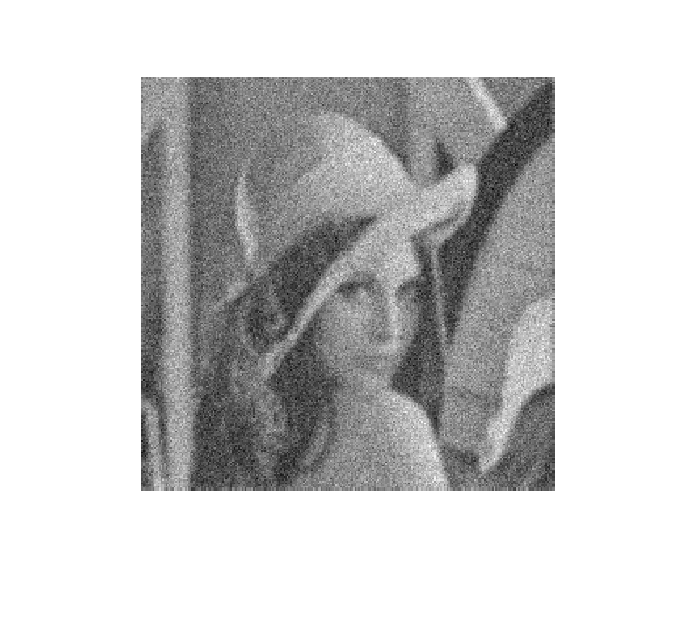
\includegraphics[width=0.45\textwidth]{../program/f.eps}
    } 
\end{figure}
\subsection{TV}
采用参数
\[  
  \mu = 1, \lambda = 0.001, maxstep = 10, tol = 1e-7, \delta = 0.1
\]
计算结果如下:
\begin{figure}[H]
  \subfigure[待处理图片]{
    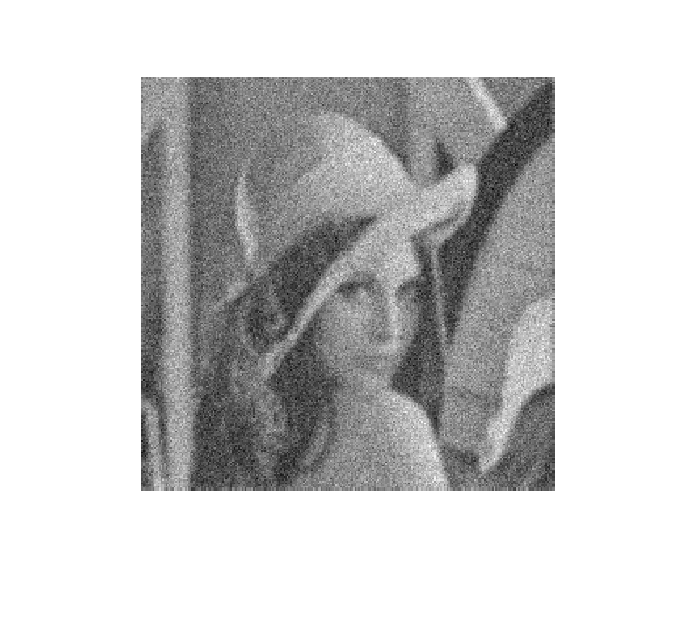
\includegraphics[width=0.45\textwidth]{../program/f.eps}
  }
  \subfigure[TV]{
    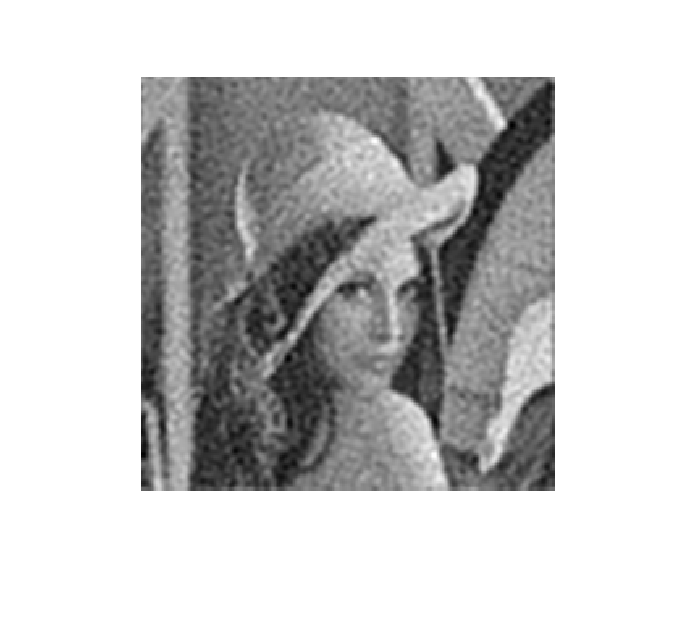
\includegraphics[width=0.45\textwidth]{../program/TV.eps}
    } 
\end{figure}
原图的相对误差为0.1987,TV处理之后图片的相对误差为0.1124.
\subsection{Analysis Based Approach}
采用参数
\[
   \mu = 0.1, \lambda = 0.01, maxstep = 10, tol = 1e-7, \delta = 0.1 
\]
小波框架的分解层数固定为2。
计算结果如下:
\begin{figure}[H]
  \subfigure[待处理图片]{
    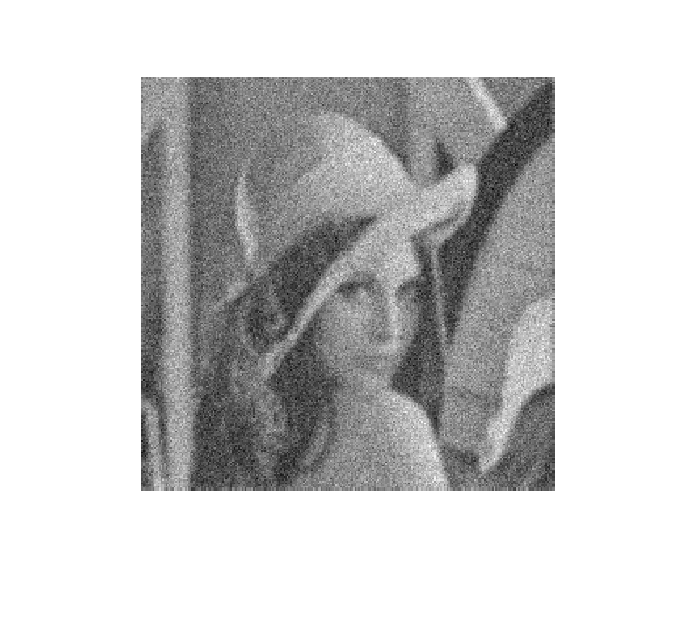
\includegraphics[width=0.45\textwidth]{../program/f.eps}
  }
  \subfigure[frame=0]{
    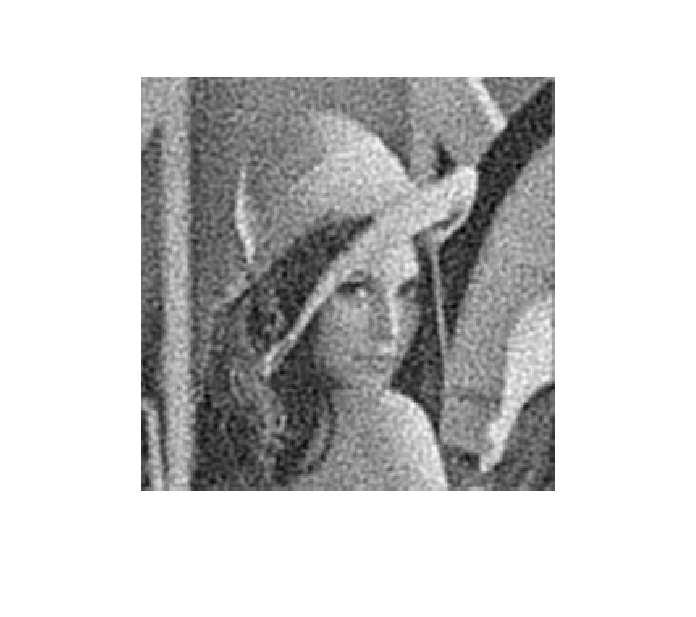
\includegraphics[width=0.45\textwidth]{../program/ADMM-0.eps}
    } 
  \subfigure[frame=1]{
    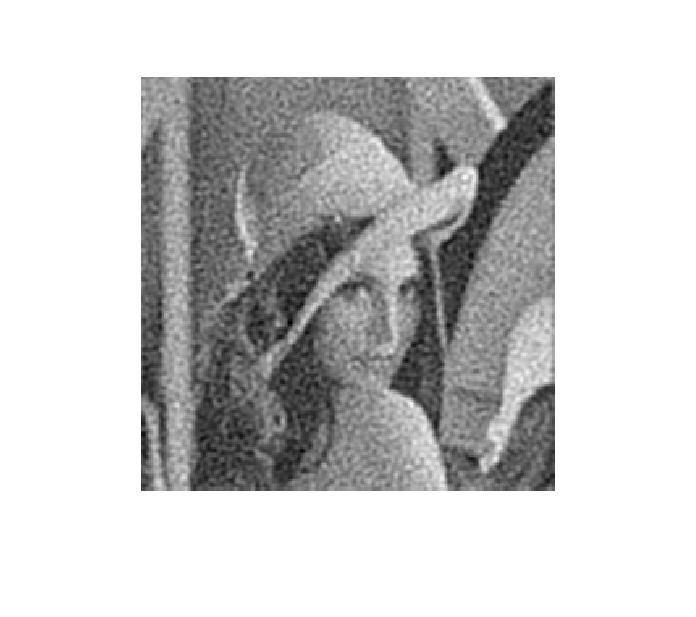
\includegraphics[width=0.45\textwidth]{../program/ADMM-1.eps}
    } 
  \subfigure[frame=3]{
    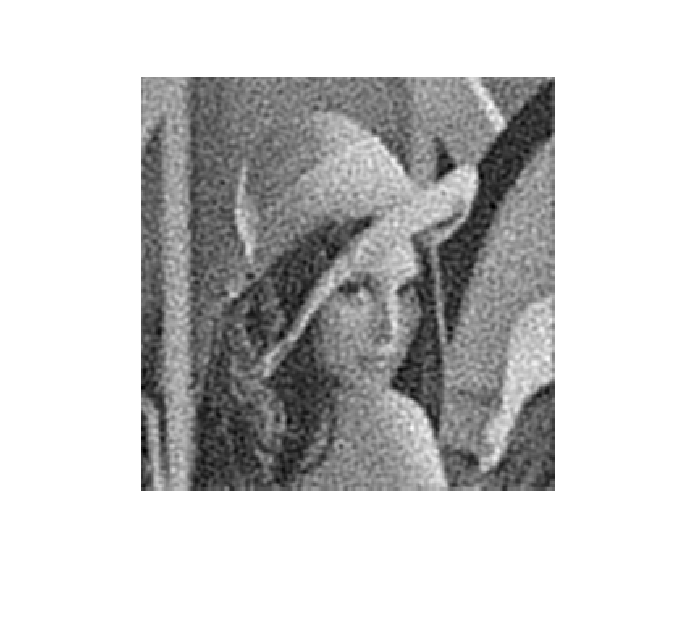
\includegraphics[width=0.45\textwidth]{../program/ADMM-3.eps}
    } 
  \end{figure}
四张图相对误差分别为0.1987,0.1563,0.1577,0.1568.
\subsection{Balanced Approach}
采用参数
\[ 
 \kappa = 1, L=10, maxstep =10, tol = 1e-7, \lambda = 100
 \]
 小波框架的分解层数固定为2。计算结果如下:
\begin{figure}[H]
  \subfigure[待处理图片]{
    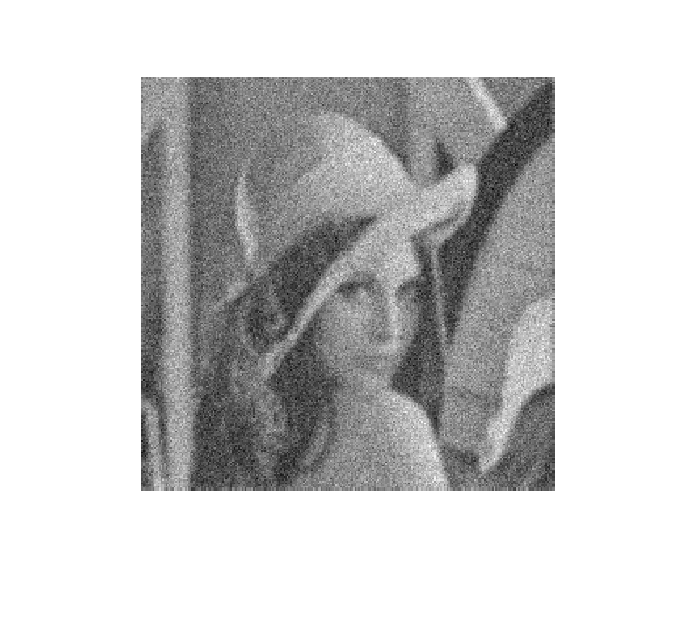
\includegraphics[width=0.45\textwidth]{../program/f.eps}
  }
  \subfigure[frame=0]{
    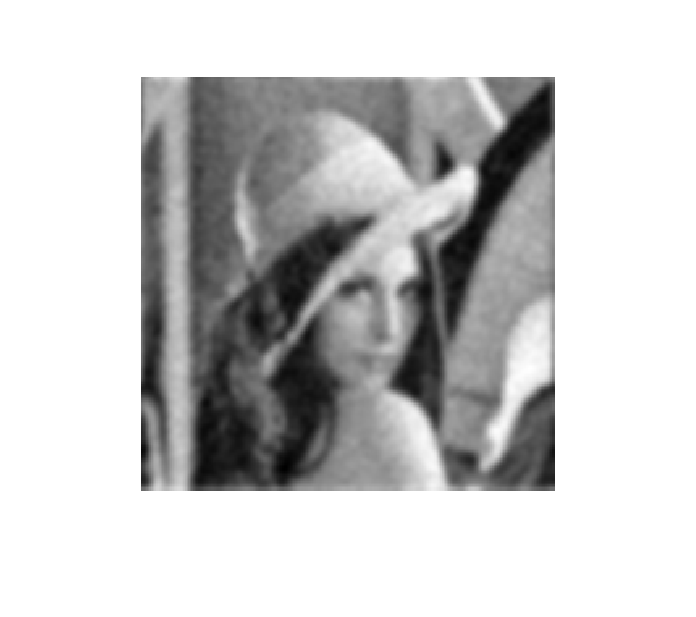
\includegraphics[width=0.45\textwidth]{../program/PFBS-0.eps}
    } 
  \subfigure[frame=1]{
    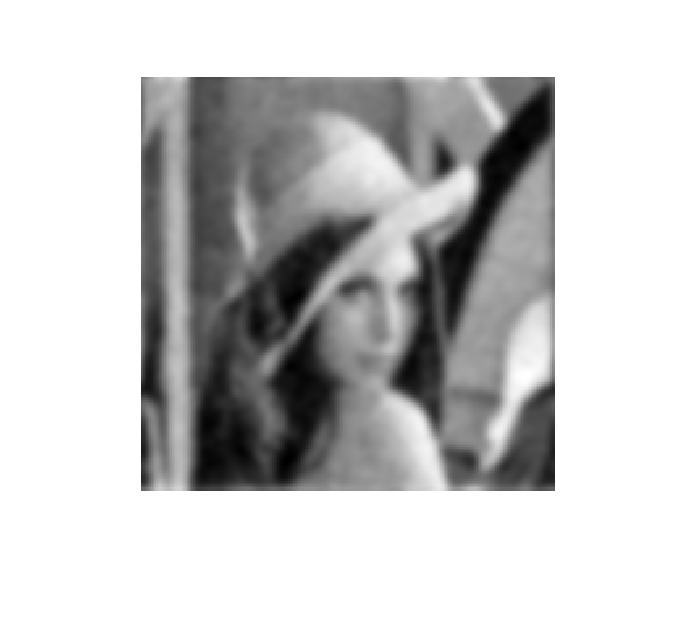
\includegraphics[width=0.45\textwidth]{../program/PFBS-1.eps}
    } 
  \subfigure[frame=3]{
    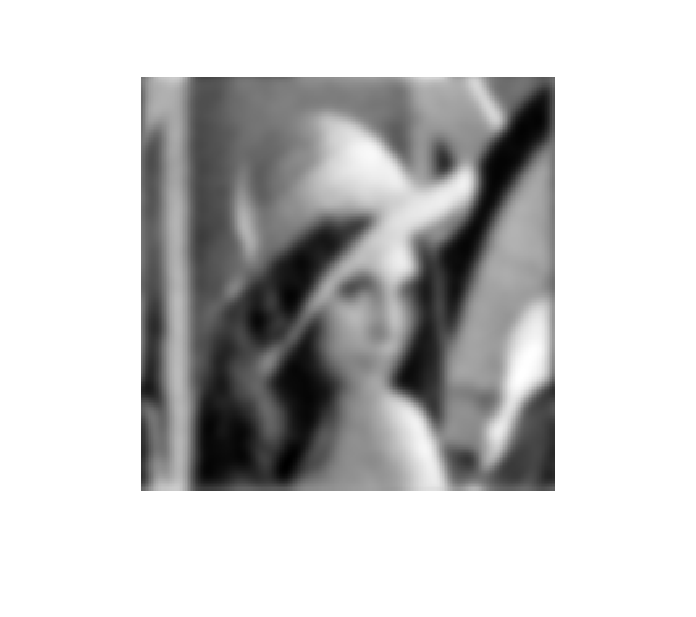
\includegraphics[width=0.45\textwidth]{../program/PFBS-3.eps}
    }
  \end{figure}
  四张图相对误差分别为0.1987,0.1289,0.1451,0.1659。

\section{上次作业总结}
本次作业我们采用小波框架的
Analysis Based Approach和 Balanced Approach 方法进行去
噪去模糊,并与之前写过的TV方法进行比较,发现从视觉感受角度而言,
Analysis Based Approach的去噪去模糊效果最佳,但从误差分析角度而言,
PFBS的效果最优,但实际感受PFBS虽然消除了噪声,但较大的增加了模糊,
使图像更难以分辨。

\end{document}
